
\section{Anotaciones sobre el modelo}

La arquitectura de red utilizada en el diseño del agente inteligente es un \textbf{Perceptron Multicapa (MLP)} como se puede ver en la figura \ref{fig:perceptronml}


\begin{itemize}
	\item 0 si está libre.
	\item 1 si está asignado a un operador.
\end{itemize}

En la figura \ref{fig:ejemploAsignacion} se puede observar un ejemplo de una asignación para una banda con 9 canales y 3 operadores.

\begin{figure}[H]
	\centering
	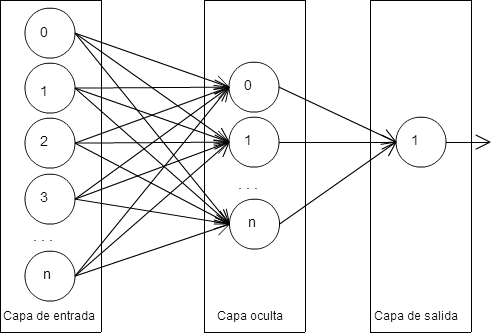
\includegraphics[width=9cm]{Capitulo4Modelo/Imagenes/redmlp.png}
	\caption{Perceptron multicapa.}
	\label{fig:perceptronml}	
\end{figure}



\section{Datos de entrada}

Las variables de entrada representan el estado actual del modelo, en otras palabras la asignación actual del espectro en una banda de interés.

\begin{itemize}
	\item $C$: Cardinalidad del conjunto de canales definidos para un servicio particular.
	\item $O$: Número de operadores en la banda que requieren asignación.
	\item $N$: Número de operadores presentes en la banda.
	\item $OPp = \{o_k: 1 \leq k \leq N\}$: Conjunto de etiquetas que representan a los operadores presentes.
	\item $OPi = \{o_k: 1 \leq k \leq O\}$: Conjunto de etiquetas que representan a los operadores que solicitan canales. Si $o_k \in OPp$, es un operador presente o antiguo; sino, es un operador nuevo.
	\item $OPt$ = $OPp \cup OPi$: Son las etiquetas de los operadores presentes en la banda y de los que requieren asignación.
	\item $CI_{c} \in \{0,1\}$: Canales marcados como inutilizables en la banda, si $CI_{c} = 1$ el canal $c$ es inutilizable, en caso contrario se puede usar, donde  $1 \leq c \leq C$.
	\item $CR_{c} \in \{0,1\}$: Canales marcados como reservados en la banda,  si $CR_{c} = 1$ el canal $c$ está reservado, en caso contrario se puede usar, donde  $1 \leq c \leq C$.
	\item $CP_{c} \in \{0,1\}$: Canales asignados en las subdivisiones de la banda,  si $CP_{c} = 1$ el canal $c$ está asignado, en caso contrario se encuentra libre, donde  $1 \leq c \leq C$.
	\item $B^{I}_{co} \in \{0,1\}$: Indica si en el canal $c$ de la banda se encuentra asignado el operador $o$ donde $1 \leq c \leq C, o \in OPp$.
	\item $Req=[(o_{1}, nr_{1}), (o_{2}, nr_{2}), ... ,(o_{O}, nr_{O})]$: $(o, nr)$ indica que el operador etiquetado $o \in OPi$ requiere $nr$ canales.
	\item $Sep$: Valor de separación mínima de canales entre canales asignados a operadores distintos.
	\item $Tope$: Valor máximo de canales que puede tener asignado un operador en una banda específica.
	\item $AP_{o}$: Indica el número máximo de canales que tiene el operador $o$ en una subdivisión de la región de trabajo, donde $1 \leq o \leq O$.
	\item $R$: Número máximo de operadores por canal. Por defecto su valor es 1.
	\item $CAC \in \{0,1\}$: Indica si se conserva asignación para operadores que solicitan nuevos canales y ya tienen asignación actualmente.
\end{itemize}


\section{Variables de decisión}

Las variables de decisión son aquellas que se desean encontrar en el problema, en este caso la asignación de canales a nivel nacional, regional, departamental o municipal.

\begin{itemize}
	\item ${B}^{O}_{co} \in \{0,1\}$ Asignación de los operadores en la banda, donde $1 \leq c \leq C, o \in OPt$
\end{itemize}


\section{Variables usadas en restricciones y estrategias de búsqueda}

Son aquellas variables que se utilizan para ayudar a definir algunas restricciones y las estrategias de búsqueda.

\begin{itemize}
	\item{$EC_{c} \in \{0,1\}$ es una variable reificada que define si el canal $c$ esta libre u ocupado.
	\begin{displaymath}
		\begin{array}{cc}
			(\forall c \in \{1,2,...,C\} ) \sum \limits_{o \in OPt} B^{O}_{co} + CP_{c} < 1 \leftrightarrow EC_{c} = 1
		\end{array}
	\end{displaymath}
	El canal $c$ se encuentra libre si y sólo si $EC_{c} = 1$}
	\item {$CAO_{co} \in \{0,1\}$: Permite conocer el número de bloques contiguos asignados a un operador $o$, de la siguiente forma:
	\begin{displaymath}
		CAO_{co} = \left\{ \begin{array}{lp{5cm}} 1  \textrm{ Si un bloque de canales asignados al operador etiquetado $o$ termina en el canal $c-1$ } \\1 \textrm{ Si un bloque de canales asignados al operador etiquetado $o$ inicia en el canal $c$ } \\0 \textrm{ En otro caso}\end{array}\right.
	\end{displaymath}	
	Si para un operador $o$ se cumple $B^{O}_{co} \neq B^{O}_{(c+1)o}$ y $c<C$ entonces $CAO_{co}=1$ en caso contrario $CAO_{co}=0$, para el caso donde $c=C$ y $B^{O}_{co}=1$ entonces $CAO_{co}=1$ en caso contrario $CAO_{co}=0$, donde: $1 \leq c \leq C, o \in OPt$.}
	\item $CLM_{c}$: Define el tamaño de los bloques libres, si $c=1$ entonces $CLM_{c}=EC_{c}$, si $c>1$ y $EC_{c}=1$ entonces  $CLM_{c}=1+CLM_{c-1}$, si $c > 1$ y $EC_{c}=0$  entonces $CLM_{c}=0$, donde $1 \leq c \leq C$.
	\item $CLMmax = max(CLM_c: 1 \leq c \leq C)$
	\item {$CAI_{c} \in \{0,1\}$: Permite conocer que canales se encuentran marcados como inutilizados debido a la separación mínima exigida entre dos operadores diferentes.
	\begin{displaymath}
		CAI_{c} = \left\{ \begin{array}{lp{5cm}} 1  \textrm{ Si el canal se encuentra a una distancia entre $1$ y $Sep$ de un canal asignado} \\0 \textrm{ En otro caso } \end{array}\right.
	\end{displaymath}		
	Para un canal $c$ y un operador $o$ si $B^{O}_{co}=1$ y $B^{O}_{(c+1)o}=0$, entonces $\forall c, 1 \leq i \leq Sep, CAI_{c+i}= 1$, en caso de que $B^{O}_{co}=1$ y $B^{O}_{(c-1)o}=0$ entonces  $\forall c, 1 \leq i \leq Sep, CAI_{c-i} = 1$, si $B^{O}_{co} = B^{O}_{(c+1)o}$ entonces $CAI_{c}=0$  . En caso de que $R>1$ o $Sep=0$, entonces $\forall c \in \{1,2,...,C\} , CAI_{c}=0$}
\end{itemize}


\section{Restricciones}

\subsection{Restricciones triviales}


Todo operador que solicita canales y actualmente tiene canales asignados los conserva a menos que $CAC \neq 1$

\begin{equation}
	\begin{array}{cc}
		CAC = 1 \to \forall c \in \{1,2,...,C\} ,o \in OPp \cap OPi, B^{I}_{co} = 1 \to  B^{O}_{co} = 1
	\end{array}
\end{equation}

Todo operador que no solicita canales tendrá la misma asignación de canales en la salida

\begin{equation}
	\begin{array}{cc}
		\forall c \in \{1,2,...,C\} , o \in OPp \setminus OPi\\
		B^{I}_{co} = B^{O}_{co}
	\end{array}
\end{equation}

Máximo R operadores por canal

\begin{equation}
	\begin{array}{cc}
		\forall c \in \{1,2,...,C\}  \sum \limits_{o \in OPt} B^{O}_{co} + CP_{c} \leq R
	\end{array}
\end{equation}

En el caso de que un canal esté reservado o marcado como inutilizable, no puede ser asignado a ningún operador que requiere asignación

\begin{equation}
	\begin{array}{cc}
		\forall c \in \{1,2,...,C\} CI_{c} + CR_{c} \geq 1 \to \sum \limits_{o \in OPi} B^{O}_{co} = 0
	\end{array}
\end{equation}

Todos los operadores que solicitan canales y no se encuentran actualmente con asignación, deben tener asignados un número de canales igual al que requieren.

\begin{equation}
	\begin{array}{cc}
		\forall o \in OPi \setminus OPp, \sum \limits^{C}_{c=1} B^{O}_{co} = Req_{o}
	\end{array}
\end{equation}

Todos los operadores que solicitan canales y actualmente tienen asignación, deben tener asignados un número de canales igual al que requieren más los canales que actualmente poseen en la banda.

\begin{equation}
	\begin{array}{cc}
		\forall o \in OPi \cap OPp, \sum \limits^{C}_{c=1}B^{O}_{co} = \sum \limits^{C}_{c=1}B^{I}_{co} + Req_{o}
	\end{array}
\end{equation}

\subsection{Restricciones co-canal}

Debe existir una distancia de $Sep$ entre dos canales asignados a operadores diferentes que solicitan asignación.

\begin{equation}
	\begin{array}{cc}
	R=1 \to (\forall o \in OPi, \forall o' \in OPt, \forall s \in \{1,2,...,Sep\}, \forall c \in \{1,2,...,C\} , o \neq o')\\(B^{O}_{co}+B^{O}_{(c \pm s)o'} \leq 1)
	\end{array}
\end{equation}

\subsection{Restricciones legales}

Un operador no puede superar el tope de canales establecido por el gobierno en una banda de la región ni en sus divisiones territoriales

\begin{equation}
	\begin{array}{cc}
	(\forall o \in OPi)\sum \limits^{C}_{c=1} B^{O}_{co} + APo_{o} \leq Tope
	\end{array}
\end{equation}


